%
% Complete documentation on the extended LaTeX markup used for Insight
% documentation is available in ``Documenting Insight'', which is part
% of the standard documentation for Insight.  It may be found online
% at:
%
%     http://www.itk.org/

\documentclass{InsightArticle}

\usepackage{cases}
\usepackage{cite}
\usepackage[dvips]{graphicx}
\usepackage{subfigure}

%%%%%%%%%%%%%%%%%%%%%%%%%%%%%%%%%%%%%%%%%%%%%%%%%%%%%%%%%%%%%%%%%%
%
%  hyperref should be the last package to be loaded.
%
%%%%%%%%%%%%%%%%%%%%%%%%%%%%%%%%%%%%%%%%%%%%%%%%%%%%%%%%%%%%%%%%%%
\usepackage[
% dvips,
pagebackref=true,
pdfhighlight=/I,
bookmarks=true,
bookmarksopen=true,
% backref=true,
colorlinks=true,
linkcolor=blue,
citecolor=blue,
urlcolor=blue,
pdfauthor={A. Gelas, A. Gouaillard,}
pdftitle={Parametrization},
pdfcenterwindow=true,
pdffitwindow=true,
hyperfigures=true
]{hyperref}
\graphicspath{{fig/}}

\def \ie {\textit{i.e. }}
\def \Border {\mathcal{B}}
\def \Neighbor {\mathcal{N}}
\def \Mesh {\mathcal{M}}
\newcommand \vect[1]{\boldsymbol{\mathrm{#1}}}
\newcommand \suml[2]{\sum\limits_{#1}^{#2}}
%  This is a template for Papers to the Insight Journal. 
%  It is comparable to a technical report format.

% The title should be descriptive enough for people to be able to find
% the relevant document. 
\title{Parametrization of Discrete Surfaces}

% Increment the release number whenever significant changes are made.
% The author and/or editor can define 'significant' however they like.
\release{0.02}

% At minimum, give your name and an email address.  You can include a
% snail-mail address if you like.
\author{Arnaud Gelas, Alexandre Gouaillard\\ and Sean Megason}
\authoraddress{Megason Lab, Department of Systems Biology,\\
Harvard Medical School, Boston, MA, USA}


\begin{document}


\ifpdf
\else
   %
   % Commands for including Graphics when using latex
   % 
   \DeclareGraphicsExtensions{.eps,.jpg,.gif,.tiff,.bmp,.png}
   \DeclareGraphicsRule{.jpg}{eps}{.jpg.bb}{`convert #1 eps:-}
   \DeclareGraphicsRule{.gif}{eps}{.gif.bb}{`convert #1 eps:-}
   \DeclareGraphicsRule{.tiff}{eps}{.tiff.bb}{`convert #1 eps:-}
   \DeclareGraphicsRule{.bmp}{eps}{.bmp.bb}{`convert #1 eps:-}
   \DeclareGraphicsRule{.png}{eps}{.png.bb}{`convert #1 eps:-}
\fi


\maketitle


\ifhtml
\chapter*{Front Matter\label{front}}
\fi


% The abstract should be a paragraph or two long, and describe the
% scope of the document.
\begin{abstract}
Parametrization of surfaces, sometimes called \emph{flattening} as it maps a surface embedded in 3D into its intrinsic 2D domain, is a powerful tool for surface analyzing, processing. For the past years, there has been a growing interest in the Community that even lead to one implementation of one special type of parametrization in ITK~\cite{Haker00a,Haker00b,Angenent99,Gao06}. We are providing here a more general framework for parametrization of single connected surfaces of any genus with fixed boundary. It is based on a recent addition to ITK: itkQuadEdgeMesh~\cite{itkQE} which allows an elegant implementation of algorithm for geometry and topology processing of discrete 2-manifolds. The 6 algorithms that we implemented map the meshes into a planar domain with fixed boundary leading to more stability and speed than mapping into the spherical domain. Each of them use different kind of parametrization with different properties. The conformal parametrization is usually used as it is intrinsic to the geometry of the mesh and thus allow shape analysis independently of the connectivity. However if flattening the mesh is your only goal, then the simplest parametrization algorithm (graph theory) will give you the best speed. This is the case when you want to further process the mesh in a lower dimension. Using sparse direct solvers, the parametrization of meshes can be done sufficiently fast (couple of seconds) to consider this approach in interactive applications. 

\noindent
% This document describes a new algorithm implemented using the Insight Toolkit
% ITK \url{www.itk.org}.  The code of the algorithm is written following the 
% ITK CodingStyle as described in the directory
% 
% \code{Insight/Documentation/Style.pdf}
% 
% This paper is accompanied with the source code, input data, parameters and
% output data that the authors used for validating the algorithm described in
% this paper. This adheres to the fundamental principle that scientific
% publications must facilitate reproducibility of the reported results.
\end{abstract}

\tableofcontents

\section{Introduction}
\subsection{Statement of the problem}

Given any two meshes with the same topology, it is possible to compute a one-to-one and onto mapping between them~\cite{Hormann:2007:MPT}. Whenever one of these two surfaces is represented by a triangular mesh, with at least one boundary and singly connected, this problem is referred as \emph{mesh parametrization}. Note that a surface without boundary can be cut open along an arbitrary path to lead to the same surface with a boundary. An algorithm to generate such a \emph{cut-graph} is already included in the itkQuadEdgeMesh \cite{itkQE} submission. Thus the problem we address with this code is much more general than the one addressed in \cite{Haker00a,Haker00b,Angenent99,Gao06} where they limit their application to genus 0 meshes, and where they map to sphere, which is known to be more unstable.

\subsection{Applications}
\begin{itemize}
    \item detail mapping, synthesis
    \item morphing, detail transfer
    \item mesh completion
    \item mesh editing
    \item remeshing
    \item compression
    \item surface fitting
    \item etc...
\end{itemize}

This problem have received a lot of interest over the two last decades. Here we will not review all of them, so we invite interested reader to have a look to~\cite{Floater:2005:SPA,Sheffer06:Survey,Hormann:2007:MPT} for recent surveys concerning all these techniques. Parametrization of surfaces has been used in brain mapping \cite{Gu04}, Colonoscopy \cite{Gu06},  cortical surface shape analysis \cite{Yu07}, vessel geometry processing and many other medical or biological problems. In this paper, we only focus on \emph{linear parametrization with fixed boundaries}.

In the following sections, we first present the required theoretical background and present in details the design of our code.

\section{Background}

\subsection{Principle}
\label{sec:ParameterizationPrinciple}

Since we only consider \emph{linear parametrization with fixed boundaries}, one can see this method as a \emph{spring and mass model} where each vertex of the mesh is a mass and each edge of the triangular mesh is a spring. By constraining the boundary of this model, the interior vertices will relax to the minimum of spring energy. 

Consider each spring is ideal, \ie the rest length is null and the potential energy is only $\frac{1}{2} Dl^2$, where $D$ is the spring constant and $l$ is the length of the spring. Then specify the desired parameter values $\vect{u}_i=(u_i,v_i)_{i=1,\ldots,L}$ for the boundary points $\vect{p}_i \in \Border$, with $L$ is the number of points on the boundary, then compute the parametrization can be computed by minimizing the following energy:
\begin{equation}
    E = \frac{1}{2}\suml{i=1}{N}\ \suml{j\in\Neighbor_i}{} \frac{1}{2} D_{ij} \|\vect{u}_i - \vect{u}_j \|^2,\label{eq:SpringEnergy}
\end{equation}
where $N$ is the number of points of the mesh, $\Neighbor_i$ is the neighborhood of the vertex $\vect{p}_i$, and $D_{ij}=D_{ji}$ is the spring constant corresponding to the edge connecting $\vect{p}_i$ and $\vect{p}_j$.

The minimization of Eq.~\ref{eq:SpringEnergy} leads to solve the following sparse linear systems
\begin{equation}
    A \cdot \vect{U} = \bar{\vect{U}}
\end{equation}
where $A$ is a $n \times n$ sparse square matrix with elements
\begin{numcases}{A_{ij} = }
   1 & if $i=j$, \nonumber \\
   -D_{ij} \left/ \suml{k\in \Neighbor_i}{}D_{ik}\right. & if $j \in \Neighbor_i$, \nonumber \\
   0 & else
\end{numcases}
$\vect{U}=(\vect{u}_i)_{i=1,\ldots,N} = (u_i,v_i)_{i=1,\ldots,N}$ is a $2 \times n$ matrix of unknown parameter values (inner points) and $\bar{\vect{U}}=(\bar{\vect{u}}_i)_{i=1,\ldots,N} = (\bar{u}_i,\bar{v}_i)_{i=1,\ldots,N}$ is a $2 \times n$  matrix with coefficients
\begin{equation}
    (\bar{u}_i,\bar{v}_i) = \suml{j\in \Neighbor_i,\ j \in \Border}{}-\frac{D_{ij}}{\suml{k\in \Neighbor_i}{}D_{ik}} (u_j, v_j)
\end{equation}

As we have just presented, considering a triangular mesh as a mass spring model with constrained boundaries, naturally leads to solve linear systems. For this reason, such kind of methods are generally referred as \emph{linear parametrizations with fixed boundaries}.

\subsection{Barycentric Weights}
\label{sec:BarycentricWeights}

\begin{figure}
\centering
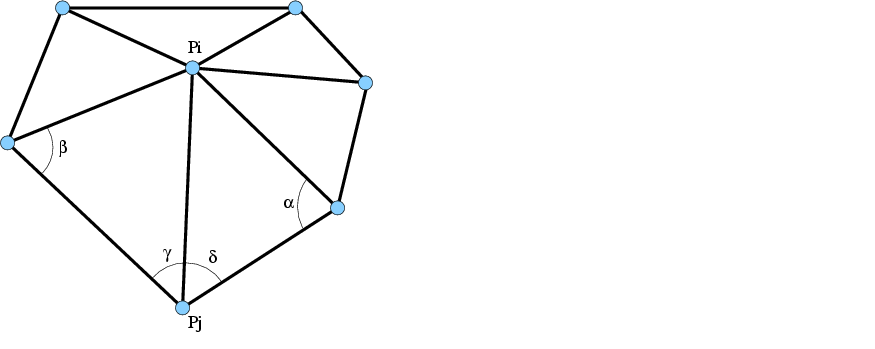
\includegraphics[width=0.6\textwidth]{param}\label{fig:angle_description}
\caption{A $3$D $1$-ring and its associated flattened version.}
\end{figure}

Now the main difference between all these methods reside in the choice of the \emph{spring constants}, \ie \emph{barycentric weights}. We provide here some of the possible choices given in the literature:
\begin{enumerate}
    \item \emph{Graph theory based}~\cite{Tutte60,Tutte63} 
\begin{equation}
    D_{ij} = 1
\end{equation}
    \item \emph{Chord Length}~\cite{} 
\begin{equation}
    D_{ij} = \frac{1}{\|\vect{p}_i - \vect{p}_j\|^2}    
\end{equation}
    \item \emph{Discrete Conformal}~\cite{pinkall93computing} 
\begin{equation}
    D_{ij} = \text{cot }\alpha_{ij} + \text{cot }\beta_{ij}
\end{equation}
    \item \emph{Discrete Authalic}~\cite{Desbrun02}
\begin{equation}
    D_{ij} = \frac{\text{cot }\gamma_{ij} + \text{cot }\delta_{ij} }{\|\vect{p}_i - \vect{p}_j\|^2}
\end{equation}
    \item \emph{Intrinsic}~\cite{Desbrun02}
\begin{equation}
    D_{ij} = \mu * \frac{\text{cot }\gamma_{ij} + \text{cot }\delta_{ij} }{\|\vect{p}_i - \vect{p}_j\|^2} + ( 1- \mu) * 
\text{cot }\alpha_{ij} + \text{cot }\beta_{ij}
\end{equation}
\end{enumerate}

\subsection{Boundary Mapping}

As presented, the first step of linear parametrizations with fixed boundary is to choose the image of the boundary points in the parametric space. 

The most common strategy is to fix the boundary points on a convex shape. Indeed it guarantees the bijectivity of the parametrization if positive barycentric weights are used. For these reasons, most of linear parametrization with fixed boundary take a square, or a circle as parameter domain.

\subsection{Numerical Issues}

As we mention previously in section~\ref{sec:ParameterizationPrinciple}, linear parametrizations with fixed boundary require to solve sparse linear systems. There are many ways to solve sparse linear systems $A\vect{x} = \vect{b}$, but all methods can be classified into two categories:
\begin{description}
\item[iterative solvers] starting from an initialized solution $\vect{x}^0$, the solution is iteratively updated until convergence to the solution $\vect{x}$. The difference between these methods reside in the way to update the solution $\vect{x}^i$. 

\item[direct solvers] factorize the matrix $A$ into a product of matrices that are simple to invert. For example, a $LU$ decomposition consists in finding the lower triangular matrix $L$ and the upper triangular matrix\footnote{If A is symmetric, then $U=L^t$ and the factorization is referred as a \emph{Cholesky} factorization.}  $U$ such that the product $LU$ is equal to A of the system to be solved. Then solving the linear system is equivalent to solve easy triangular systems, \ie
\begin{numcases}{A\vect{x} = \vect{b}\  \Leftrightarrow\  LU\vect{x} = \vect{b}\  \rightarrow\  }
    L\cdot\vect{y} = \vect{b} \nonumber \\
    U\cdot\vect{x} = \vect{y} \nonumber 
\end{numcases}
\end{description}

A nice study has been done \cite{Kobbelt05} that illustrates the advantages and inconvenients of the multitude of solvers available in the case of mesh processing. This comparative study have showed that sparse direct solvers are much faster than iterative ones. Moreover with using iterative solvers, a special attention is required on the matrix conditioning, and thus generally requires a preconditioning.

We decided that it would be better not to hard code the choice of the solver in the code. First because that would mean hard coding the usage of the vnl solver, the only sparse linear solver available to ITK by default. Unfortunately nowadays, vnl only provides iterative methods for solving sparse linear system, and is thus much slower than direct one available. Second because whichever solver is faster today might not be the fastest next year given how fast the research on that field seems to be recently. We took an a-la C-GAL approach where the code is templated over the solver, even if our implementation then differs from C-GAL in many ways.

\section{Design}

Following the previous section, the design of the code is straightforward, each functionality should be independent in order to make the use of the class as flexible as possible. The design of our class is finally given in Fig.~\ref{fig:class_design}.

\begin{figure}[htbp]
    \centering
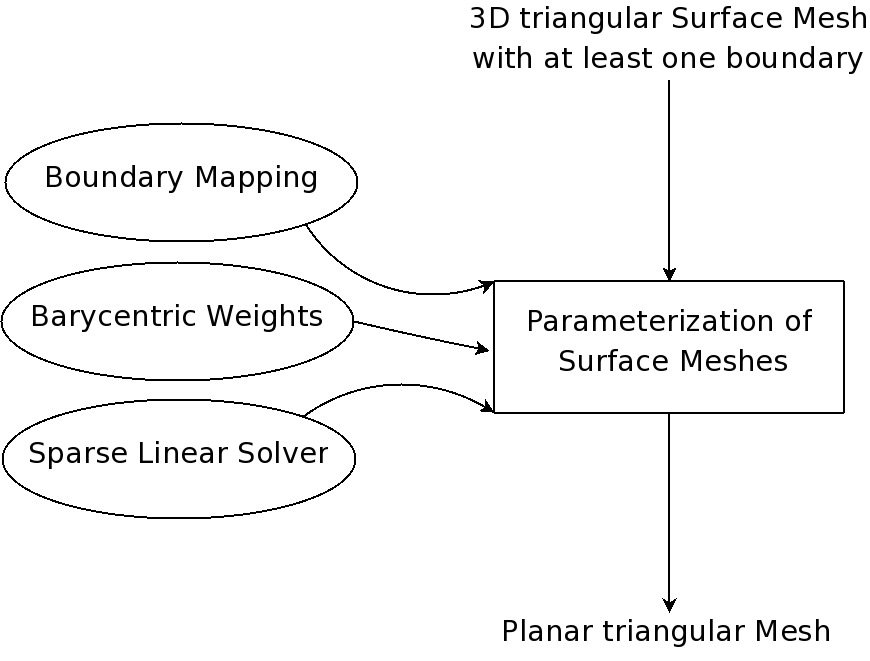
\includegraphics[width=0.5\textwidth]{Diagram1}
\caption{Design of our implementation. The parametrization class takes as input a $3$D Surface Mesh $\Mesh$ with at least one boundary, and the choice of the boundary mapping and the barycentric weights is made through the corresponding templates. It solves the resulting sparse linear systems using the solver given as a template. Its outputs a planar Mesh which is the mapping of $\Mesh$ onto the parametric domain defined by the boundary mapping, given the barycentric weights.}\label{fig:class_design}
\end{figure}

\subsection{Border Transform}

We create an abstract class \code{itk::MeshBorderTransform} which defines the API of the border transform. All derived class must contain one method to provide a border map, and the boundary mapping from the 3D space onto the parametric domain, \ie a 2D domain.

We provide two implementations of this abstract class for a square shaped domain and a a circle shaped domain.

\subsection{Barycentric weights}

For the barycentric weights, we define an abstract functor \code{itk::MatrixCoefficients}. It takes as input a $3$D triangular mesh and one half edge and return the barycentric weight corresponding to the given edge.
All the existing functors are defined in \code{itkQEMeshParamMatrixCoeficients.h}:

\begin{itemize}
    \item Graph theory based \code{class OnesMatrixCoefficients}
    \item Chord Length \code{class InverseEuclideanDistanceMatrixCoefficients}
    \item Discrete Conformal \code{class ConformalMatrixCoefficients}
    \item Discrete Authalic \code{class AuthalicMatrixCoefficients}
    \item Intrinsic \code{class IntrinsicMatrixCoefficients}
    \item Harmonic  \code{class HarmonicMatrixCoefficients}
\end{itemize}

\subsection{Parametrization}

The parametrization itself is just a mater of building the sparse systems depending on the connectivity of the surface mesh and the barycentric weights. It will delegates solving the matrix to the solver specified in the template, and then rebuild a mesh from the solution given by the solver.

\subsection{Solving sparse linear system}

\subsubsection{Iterative solvers}
Only a few parameters need to be modified in the solver. The solvers stops when the residual error is lower than a threshold or when the maximum number of iteration is reached. If the result is not satisfactory, there is great chance that the number of iterations was not set high enough. You can set a new one using \code{SetNumberOfIterations()}.

\subsubsection{Direct solvers}
No parameters are required.

\section{Software Requirements}

You need to have the following software installed:

% The {itemize} environment uses a bullet for each \item.  If you want the 
% \item's numbered, use the {enumerate} environment instead.
\begin{itemize}
  \item  Insight Toolkit 3.4 (with Review enabled)
  \item  CMake 2.4
\end{itemize}

For the sake of simplicity, we create some specific traits for solving sparse linear systems. One can either use the one we wrote, or write this own one (if you want to use any other sparse direct solver for example) and follow the same principle.

\subsection{Solvers}

vnl being included in ITK, we provide a default trait for vnl. It is strongly suggested that the user use other solvers to have an interactive experience with parametrization. vnl should only be used as a proof-of-concept or if your input mesh is relatively small. We recommend TAUCS, for which we provide traits. Both should give you the same results or better with an increase of an order of magnitude in speed.
%\url{http://www.insightsoftwareconsortium.org/wiki/index.php/IJ-Testing-Environment}

%\subsubsection{TAUCS}

Download and install TAUCS from the following page:
\url{http://www.tau.ac.il/~stoledo/taucs/}

%\subsubsection{CHOLMOD}

\section{Example}
The example given along this paper use \code{itkVTKPolyDataReader} for reading its input. If you don't have a mesh to test with, you can find many here:
\url{http://www.aim-at-shape.net}
By default, if several borders are present, the longer one is chosen. If run without arguments, the example displays its usage.

\section{Future work}

We hope that the code will make it into the ITK toolkit. Even if the code is clean and commented, it does not completely follows ITK development guide. For example we did not check the style using KWStyle; a file can contain several classes; the naming convention is not always respected, \textit{etc.}. It's all minor and the API should remain stable which motivated our early submission to the IJ.
The parametrization package open the way to remeshing techniques, and to shape matching algorithms that we would like to evaluate.
itkQuadEdgeMesh also allows a lot of mesh processing algorithm to be implemented in an elegant and optimized fashion. We are planning to implement more and more of those starting with some decimation and smoothing algorithms.

% The preceding sections will have been written in a gentler,
% introductory style.  You may also wish to include a reference
% section, documenting all the functions/exceptions/constants.
% Often, these will be placed in separate files and input like this:

%%%%%%%%%%%%%%%%%%%%%%%%%%%%%%%%%%%%%%%%%
%
%  Insert the bibliography using BibTeX
%
%%%%%%%%%%%%%%%%%%%%%%%%%%%%%%%%%%%%%%%%%

\bibliographystyle{plain}
\bibliography{parameterization_biblio}


%%%%%%%%%%%%%%%%%%%%%%%%%%%%%%%%%%%%%%%%%
%
% Appendix
%
%%%%%%%%%%%%%%%%%%%%%%%%%%%%%%%%%%%%%%%%%
%\appendix
%
%\section{This is an Appendix}
%
%To create an appendix in a Insight HOWTO document, use markup like
%this:
%
%\begin{verbatim}
%\appendix
%
%\section{This is an Appendix}
%
%To create an appendix in a Insight HOWTO document, ....
%
%
%\section{This is another}
%
%Just add another \section{}, but don't say \appendix again.
%\end{verbatim}





\end{document}

